\documentclass[11pt, a4paper]{paper}
\usepackage{amsmath}
\usepackage{graphicx}
%\usepackage{subfig}

\title {\bf Jaal:: An Dual Tree Matching Approach to High Quality All-Quads Surface Meshing  } 
\author {
Chaman Singh Verma\thanks{csverma@cs.wisc.edu}, Tim Taugtes \thanks{tautges@mcs.anl.gov} }

\begin{document}
\maketitle
\abstract { 
Applications of All-Quad surface mesh are abound, as well as literature to generate and edit 
them, but to the best of our knowledge, there does not exist any high quality public domain 
all-quads mesh implementation even for complex 2D domains. 

We plan to implement a sinple and reliable all-quad mesh algorithm which is
suitable for spectral finite elements analysis.  Among various techniques that have been 
proposed in the past, we will use {\em triangle to quad} transformation which is probably the
easiest, intuitive, and most importantly, robust. Our quad meshing algorithm
has two independent components (1) Suneeta's tree mathching algorithm which combines trianngles
into quads, but we relax convexity condition from Suneeta's all quad meshing algorithm
(2) After generating topologically an {\em All Quad Mesh} using matching algorithm, we improve the 
resulting mesh using simple clean-up operations, and quadrilateral shape optimization libaries.

This All Quad Mesh algorithm is part of MOAB toolkit, which is an open source library supporting mesh 
infrastructure for petacscale field simulations.

We demonstrate the effectivness of our implementationfor both CAD and non-CAD geometrical models.
Initial experiments shows that our implementation is at least 100 times faster than the original
implementation of Suneeta's algorithm for generating topological correct mesh. Performance with
all the cleanup operations and optimization is also within some reasonable limits for some of the 
benchmarking models.
}

\section { Introduction }
Quadrilateral mesh generation have been used since late 70s by many commerical 
CFD codes and by computer graphics communities for texture applications. 
The importance of unstructured quadrilateral mesh for the complex 
geometries is well known, but it is extremely surprising to  know that 
(to the best of our knowledge) that there does not exist any open source 
all-quads surface meshing algorithm at par with highly visible unstructured 
triangular mesh i.e. {\em Triangle }. \cite{jonathan}

Quadrilateral mesh generation is probably hard problems as it does not have 
a theoretically  strong backup as a trinagle mesh generation. Still,  we strongly 
believe that it is possible to engineering an all-quads meshing algorithm  by 
integrating components; a set of heurtistics, known algorithms and optimization libraries 
that can produce an extremely high quality quadrilateral mesh for most of models of 
practical importance, if not all. 

In this work, we focus on {\em Triangle to Quad} transformation approach because 
of its simplicity and robustness. Our method is based on Suneeta's tree
matching algorithm, but we relax the convexity conditions in her algorithm and
instead of using {|em Q-Percolation Algorithm}, we use a slightly less
efficient {\em Percolation-Up } algorithm because we believe that mesh
generation and quality improvement must be two independent componenents in the
mesh generation toolkits. Once we have topologically acceptable quad mesh,
we apply simple {|em Quads CleanUp } operations and shape optimization library
{\em Mesquite} to improve the resulting mesh.

The rest of the paper is organized as follows: Section 1, describes Triangle to Quad 
tranformation using graph and tree matching algorithms. Section 2, descibes improving 
topologically correct but geometrically unacceptable quadrilateral mesh. Section 3 
describes results for both CAD and non-CAD geometrical models.
Section 4. describes implementation details and finally in Section 5, we conclude this work.

% \begin{figure}
% \begin{center}
% \includegraphics[scale=0.4]{quadflow.eps}
% \caption{There are seven independent components in developing high quality all-quad meshing algorithm.}
% \end{center}
% \label{fig:flowchart}
%\end{figure} 

\section {Previous work on all-quad meshing algorithms}

Quadrilateral mesh generation can be broadly classified into two categories
(1) Direct Methods (2) Indirect Methods. Indirect methods relies on some
background mesh ( mostly triangle ) which guide quadrilateral mesh
generation. These methods exploits the maturity of high quality triangle
mesh generators in both 2D and 3D domains and delegate the inherent complexities 
of geometric representation of the models to the triangle mesh generators. 
Direct methods on the other
hand, work directly on the geometric model without the aid of any background
mesh. They have the advantage of producing extremely high quality mesh in most
of the cases, but the computational complexities are too high and reliablity 
often is a concern.

Some techniques for all-quads meshing that are available in the literature
are:

\begin{itemize}
\item {\em Triangle to Quad-Transformation:}
Generating a topological quadrilateral mesh from a triangle mesh 
without considering the quality is extremely simple \cite{suneeta}. Just by 
adding {\em Steiner Points } at the centroid and each of three edges of the triangle
will generate three quadrilaterals as shown in the figure
\ref{fig:simplequad}. Although the algorithm is simple, the resulting
quadrilateral mesh has extremely poor quality which could be unsuitable for many
applications.
{\em Paving} The paving algorithm \cite{cass,ted} is a tightly controlled
progressive boundary algorithm. This technqiue generates a finite element mesh
by iteratively layering rows of elements along the interior of a region until
the entire object is meshed. The major challenge in this algorithm is to
produce high quality mesh when the paving boundaries collide.  
{\em Q-Morph} circumvents the difficulties of paving algorithm near the front
collision regions by using background triangle mesh. Triangles are combined to
form quadrilaterals of given shapes and sizes. This also has some problem near
the collision ....... "expand here ".
{\em Graph Matching}
Graph matching algorithms \cite{edmonds}, \cite{suneeta} pairs neighbouring
triangles to define a single quadrilaterals, this method seeks pairing
combinations that will couple every element with another. The {\em maximum
cardinality matching} is the problem of finding maximum such matchings. A {\em
perfect matching } in a graph $G$ is a subset of edges such that each node
in $G$ is met by exactly one edge if the subset. Given a real weigth $w_e$ for
every edge $e$ of $G$, the {\em minimum weight perfect-matching problem} is to
find a perfect matching $M$ of minimum weight. One of the fundamental results
in combinatorial optimization is the polynomial-time {\em Blooson} algorithm
for computing minimum-weight pefect matching by Edmonds. 

\item {\em Surface Parameterization } Surface parameterization have been
extensively studied for computer graphics applications. A nice survey is
presented by Alliez et.al. \cite{alliez}
The method of Boier-Martin et al. [2004] clusters the surface into macropatches 
and parameterizes each surface patch. Kharevych et al. [2006] find a conformal
parameterization via circle patterns. In contrast to Gu and Yau, they use
cone-singularities to increase the flexibility of purely conformal mappings. 
Dong et al. [2006] compute the Morse-Smale complex of eigenfunctions of the mesh 
Laplacian to compute a patch layout. The nodes of the complex are then utilized 
similarly to the cone singularities in [Kharevych et al., 2006].  Early approaches 
for quadrangular remeshing guided by principal curvature directions are from 
Alliez et al. [2003]. They were extended by Marinov and Kobbelt [2004], and base on 
the integration of curvature lines on the surface. Dong et al. [2005b] presented an 
algorithm which traces isolines in two conjugate harmonic vector fields. Marinov and 
Kobbelt [2006] focus on creating coarse quad-dominant meshes by approximating the 
surface with very few patches, which are then individually subdivided into quads.
Tong et al. [2006] use harmonic one-forms for surface parameterization. They 
enlarge the space of harmonic one-forms by allowing additional singular points on 
the surface. 
QuadCover is an algorithm to compute a global continuous parameterization
for an arbitrary given simplicial 2-manifold. The algorithm runs 
automatically and the parameter lines align optimally with a user-defined frame field, 
for example, the principal curvature directions.


\item {\em Spectral Quadrangulation }
Garland et.al \cite{garland} proposed spectral method for surface
quadrangulation over a triangulaed maninfold of arbitrary genus. This
apporach is based on the Morse theorem that for almost all real functions,
the Morse-Smale complex consisting of the ridge lines that extends from
its saaddle to its extrema, forms fully conforming semi-regular quadrangular 
regions. The main challenges in this approaches are (1) Selecting Morse
function (2) Solving large eigenvalue problem (3) Shifting eigenvalues on the
feature lines (4) Traversing ridge lines. All these steps are non-trivial to
implement.
\item {\em Quad-Dominated }


\item {\em Circle Packing }
In this method, before constructing a mesh, the domain is filled with closely
packed circles. The geodesic Voronoi diagram of the points of the tangencies
of these circle forms a quadrilateral mesh with $O(n log n)$ time complexity.

\end {itemize}

{\em Mesh Cleanup}
Most of the algorithms produce quad mesh with suboptimal quality and it is
often necessary to cleanup the mesh.Topological and geometric improvement
methods were presented by {Staten and Canann 1997; Kin- ney 1997 which 
results in simplified models; however, it does not provide a controllable 
means to reduce element counts in the final mesh. Another improvement 
technique [Bremer et al. 2002], developed to augment vertex valences on
grafted surfaces, uses a ring collapse methods. Related quadrilateral 
coarsening approaches have also exploited the ring structure, developing 
restructuring [Staten et al. 2008] and localized deletion techniques 
[Dewey 2008].

% Advancing front Recombination ( QMorph ) 
% ... ( Paving )
% Circle packing 
%Spectral Patches
% Global Parameterization
%Disk patches
% Graph Matching.
% Statement of Observations
%   Complexity and Functionality.
% Graph Matching 
%  Edmonds  
%  Suneeta
% Jaal: State its complexity.
%     Relaxation of Convexity
%     Bounded Quality.
% Implementation
%      Comp. Inden. of ( Tri, Global and 3D Alg.).
% Results
%      Fastest Known Implementation.
%      Robustness 2D/3D
% Conclusions
% Future Work.
%      Suneeta's Complexity estimation.

\section { Graph Matching Algorithm }
Assume we have a simple triangulated mesh $M $ i.e. every edge is shared by at most two faces which can
be converted into a graph $G = (V,E)$ with $V$ as the set of nodes and $E$ as
the set of edges.  



\begin{figure}
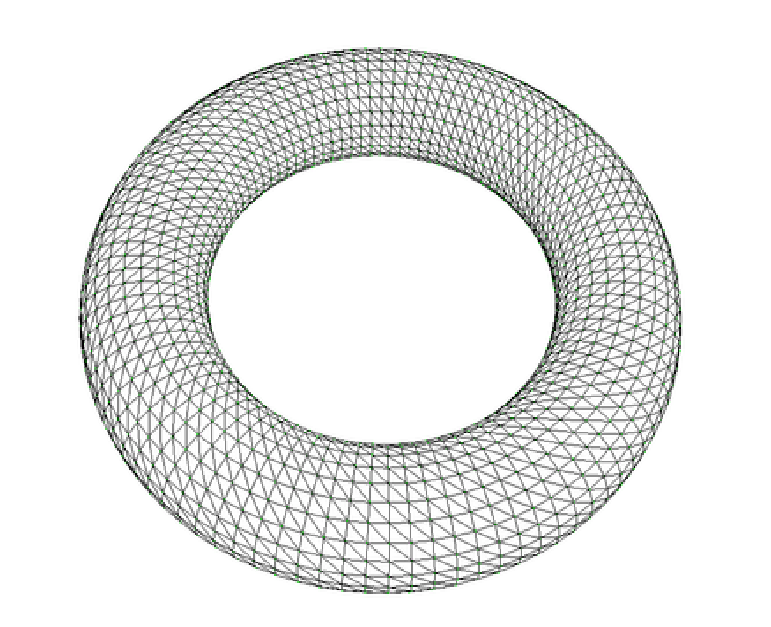
\includegraphics[scale=0.33]{torus1.eps}
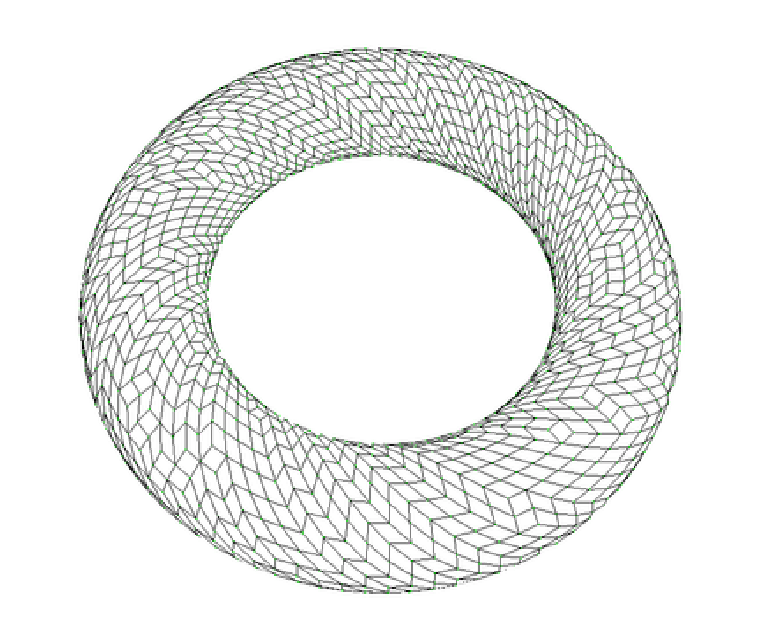
\includegraphics[scale=0.33]{torus2.eps}
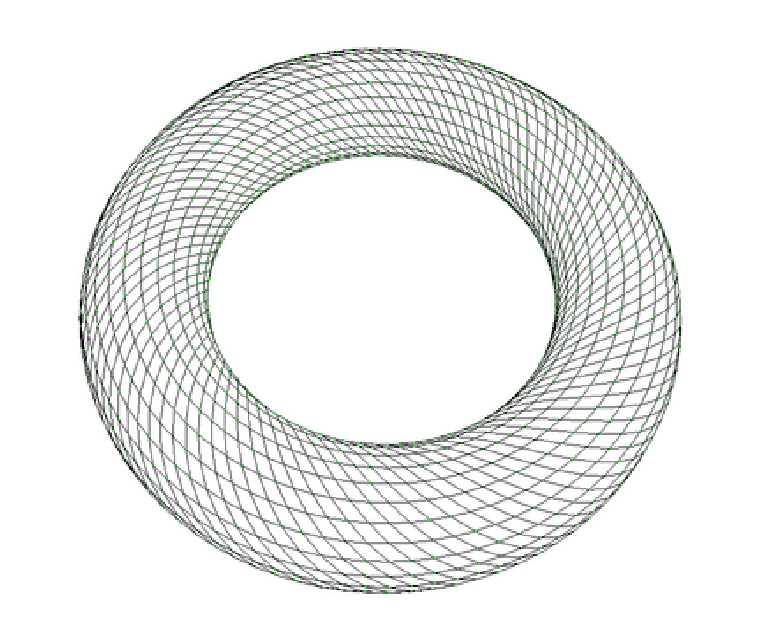
\includegraphics[scale=0.33]{torus3.eps}
\caption { (A) Input Triangle Mesh. (B) Quad Mesh using Edmonds Generalized
Graph Matching Algorithm (C) Quad Mesh using simplified Tree Matching Algorithm }
\end{figure}

\begin{table}[h]
\begin{center}
\begin{tabular}{|l|c|c|c|c|c|c|c|c|} 
\hline Model  & \multicolumn{2}{c|}{Input Mesh} & \multicolumn{3}{c|} {Graph Matching} & \multicolumn{3}{c|}{Tree Matching}  \\ \hline
\hline        & \# of  & \# of  & \# of &  \# of  & CPU    &  \# of   & \# of    & CPU      \\
              &  Nodes &  Tri  &  Nodes &  Quads  & Cycles &   Nodes  &  Quads   & Cycles   \\
\hline 
\hline Plane  &  66049 &  131072 &  66049 &  65536 & 1.058E+11   &  66049   &  65536   & 3.729E+09 \\
\hline Sphere &  40962 &   81920 &  40962 &  40960 & 1.761E+11   &  41088   &  41086   & 2.539E+09 \\
\hline Torus  &  50000 &  100000 &  50000 &  50000 & 2.695E+10   &  50000   &  50000   & 2.385E+09 \\
\hline Bunny   &  34834 &  69451 &  34834 & 34726 & 1.944E+10 &  35697 &  35588 &  2.402E+09 \\
\hline Hand    &  50085 &  99999 &  50085 & 50000 & 5.134E+10 &  53131 &  53045 &  4.043E+09  \\
\hline CAD     &  5096 &  10224 &  5096 &  5112 &  7.627E+08 &  5297 &  5313 & 2.444E+08 \\
\hline Statue  &  187644 &  375284 &  187644 & 187642 & 1.284E+12 &  189712 &  189710 &  1.246E+10 \\
\hline Art     &  241607 &  483226 &  241607 & 241613 & 8.729E+11 &  251280 &  251286 &  2.692E+10\\
\hline
\end{tabular}
\caption{Comparision of performance of Edmond's Perfect Graph Matching and 
         Sunteeta's approximate Tree Matching Algorithms }
\end{center}
\end{table}

\begin{table}[h]
\begin{center}
\begin{tabular}{|c|c|c|} 
\hline \# of Triangles &  Edmond's       & Suneeta's     \\
               & Perfect Graph Matching  & Tree Matching  \\ 
\hline  320    &   7.755E+06             & 5.636E+06      \\
\hline  1280   &   4.685E+07             & 2.263E+07       \\
\hline  5120   &   4.885E+08             & 1.266E+08       \\
\hline  20480  &   1.048E+10             & 5.642E+08       \\
\hline  81920  &   1.767E+11             & 2.575E+09       \\
\hline  327680 &      -                  & 1.371E+10       \\
\hline  1310720 &      -                 & 2.033E+11       \\
\hline
\end{tabular}
\end{center}
\end{table}






%\begin{figure}
% \begin{center}
% \includegraphics[scale=0.5]{graphtree.eps}
% %\includegraphics[scale=0.4]{dfs.eps}
% %\includegraphics[scale=0.4]{bfs.eps}
% \caption{Converting Graph into a tree.}
% \end{center}
% \label{fig:graph_tree}
%\end{figure} 

\section { Topological Clean-up}
\subsection{ Quadrilateral Convexity }
\subsection{ Basic Operations}
\subsubsection{ Face Closing }
\subsubsection{ Face Opening }
\subsubsection{ Face Swapping }
\subsection { Advancing front clean-up}
\subsection { Boundary improvement}
\subsection { Volume Preserving Laplacian Smoothing}
\section {Results}
\section { Implementation details }

\section {Conclusions}
\end{document}
